\chapter{Inleiding}
\label{inleiding}
%%%%%%%%%%%%%%%%%%%%%%%%%%%%%%%%%%%%%%%%%%%%%%%%%%%%%%%%%%%%%%%%%%%%%%%%

\begin{center}
    \begin{minipage}{0.5\textwidth}
        \begin{small}
            Waar de reden tot creatie van dit verslag worden blootgelegd, de
            opdracht en het probleem worden beschreven en achtergrondinformatie
            word gegeven.
        \end{small}
    \end{minipage}
    \vspace{0.5cm}
\end{center}

\noindent EV Europe is een bedrijf dat werkt met klanten die gebruik willen
maken van de nieuwste technieken op het gebied van elektrische auto's. Zo word
er vaak door de klanten gevraagd of moderne snufjes kunnen woorden ingebouwd in
hun auto. Recent was dat de vraag om langs de snelweg aan een snel laad paal te
kunnen laadden. Deze palen (of \ac{evse}) maken in europa gebruik van het \ac{ccs}
protocol \cite{Directive_2014/94/EU}. Dus EV Europe is gaan onderzoeken of het
gebruik van deze \ac{ccs} snel laad palen een optie is voor de klanten en wat er
voor nodig is om dit te bereiken.

%%%%%%%%%%%%%%%%%%%%%%%%%%%%%%%%%%%%%%%%%%%%%%%%%%%%%%%%%%%%%%%%%%%%%%%%
\section{Achtergrond electrichen auto's}
%%%%%%%%%%%%%%%%%%%%%%%%%%%%%%%%%%%%%%%%%%%%%%%%%%%%%%%%%%%%%%%%%%%%%%%%

Er zijn grofweg twee soorten electrice autos (\ac{ev}), plug-in elektrische auto's en
hybride auto's. Plug-in elektrische auto's zijn auto's die aleen electrise
rijden, en hybride auto's zijn auto's die zowel electrich en op
verbrandingsmotor rijden (er zijn nog meer onnderschijdingen zoals onderandenen
plug-in hybrid en waterstof autos die niet van toepassing zijn op dit verslag).

EV Europe is vooral geïnterneerd in de eerste soort, de plug-in elektrische
auto's. De plug-in elektrische auto's zijn auto's met een volledig elektrische
aandrijflijn, en die dus ook elektrisch moeten woorden opgeladen. De
aandrijflijn van deze auto's bestaat uit een accupakket, een motorcontroller,
en een elektromotor. De overigen mechanische componenten van de aandrijflijn
zijn vrijwel gelijk aan die van een interne verbrandingsmotor auto.

In de laatset jaaren is de hoeveelhijd electriche autos op de markt hard aan
het groeien. Tevens de infrastruktuur, zoals (snel)laaders. 

%%%%%%%%%%%%%%%%%%%%%%%%%%%%%%%%%%%%%%%%%%%%%%%%%%%%%%%%%%%%%%%%%%%%%%%%
\subsection{Laadden van elektricien auto's}
%%%%%%%%%%%%%%%%%%%%%%%%%%%%%%%%%%%%%%%%%%%%%%%%%%%%%%%%%%%%%%%%%%%%%%%%

Het laaden van EV's gaat wereldwijd door middel van verschillende standaarden,
maar in europa hebben het \ac{ccs} systeem geadopteerd. Ondanks de andere
standaarden die nogsteeds hier en daar ondersteund woorden, focusen we ons in
de verslag volledig op de \ac{ccs} systeem.

%%%%%%%%%%%%%%%%%%%%%%%%%%%%%%%%%%%%%%%%%%%%%%%%%%%%%%%%%%%%%%%%%%%%%%%%
\subsection{\ac{ccs} laadden}
%%%%%%%%%%%%%%%%%%%%%%%%%%%%%%%%%%%%%%%%%%%%%%%%%%%%%%%%%%%%%%%%%%%%%%%%

\ac{ccs} laaden kan met AC en met DC, afhankelijk van de \ac{evse} en de opties
op de auto kan er AC of DC woorden gelaaden. AC laaden staat wel beschreven in
de \ac{ccs} standaard, echter word het ac laaden met de type 2 stekker vaak
niet \ac{ccs} genoemd maar gewoon AC. Er zijn dus twee soorten \ac{ccs}
laadden: AC en DC.

Er zijn ook twee soorten stekkers (de kant van de \ac{evse}) en twee soorten
inlest (de kant van de \ac{ev}). de Combo 2 stekker (zie figuur
\ref{fig:CCS_combo2_outlet}) ondersteund aleen DC laaden, maar de Combo 2 inlet
(zie figuur \ref{fig:CCS_combo2_inlet}) ondersteund over het algemeen zowel AC
als DC laad. verder zijn de type 2 stekker (zie figuur
\ref{fig:AC_type2_inlet_outlet}) en inlet (zie figuur
\ref{fig:AC_type2_inlet_outlet}) alleen voor AC laaden

\begin{figure}[h]
    \centering
    \begin{minipage}{0.45\textwidth}
        \centerline{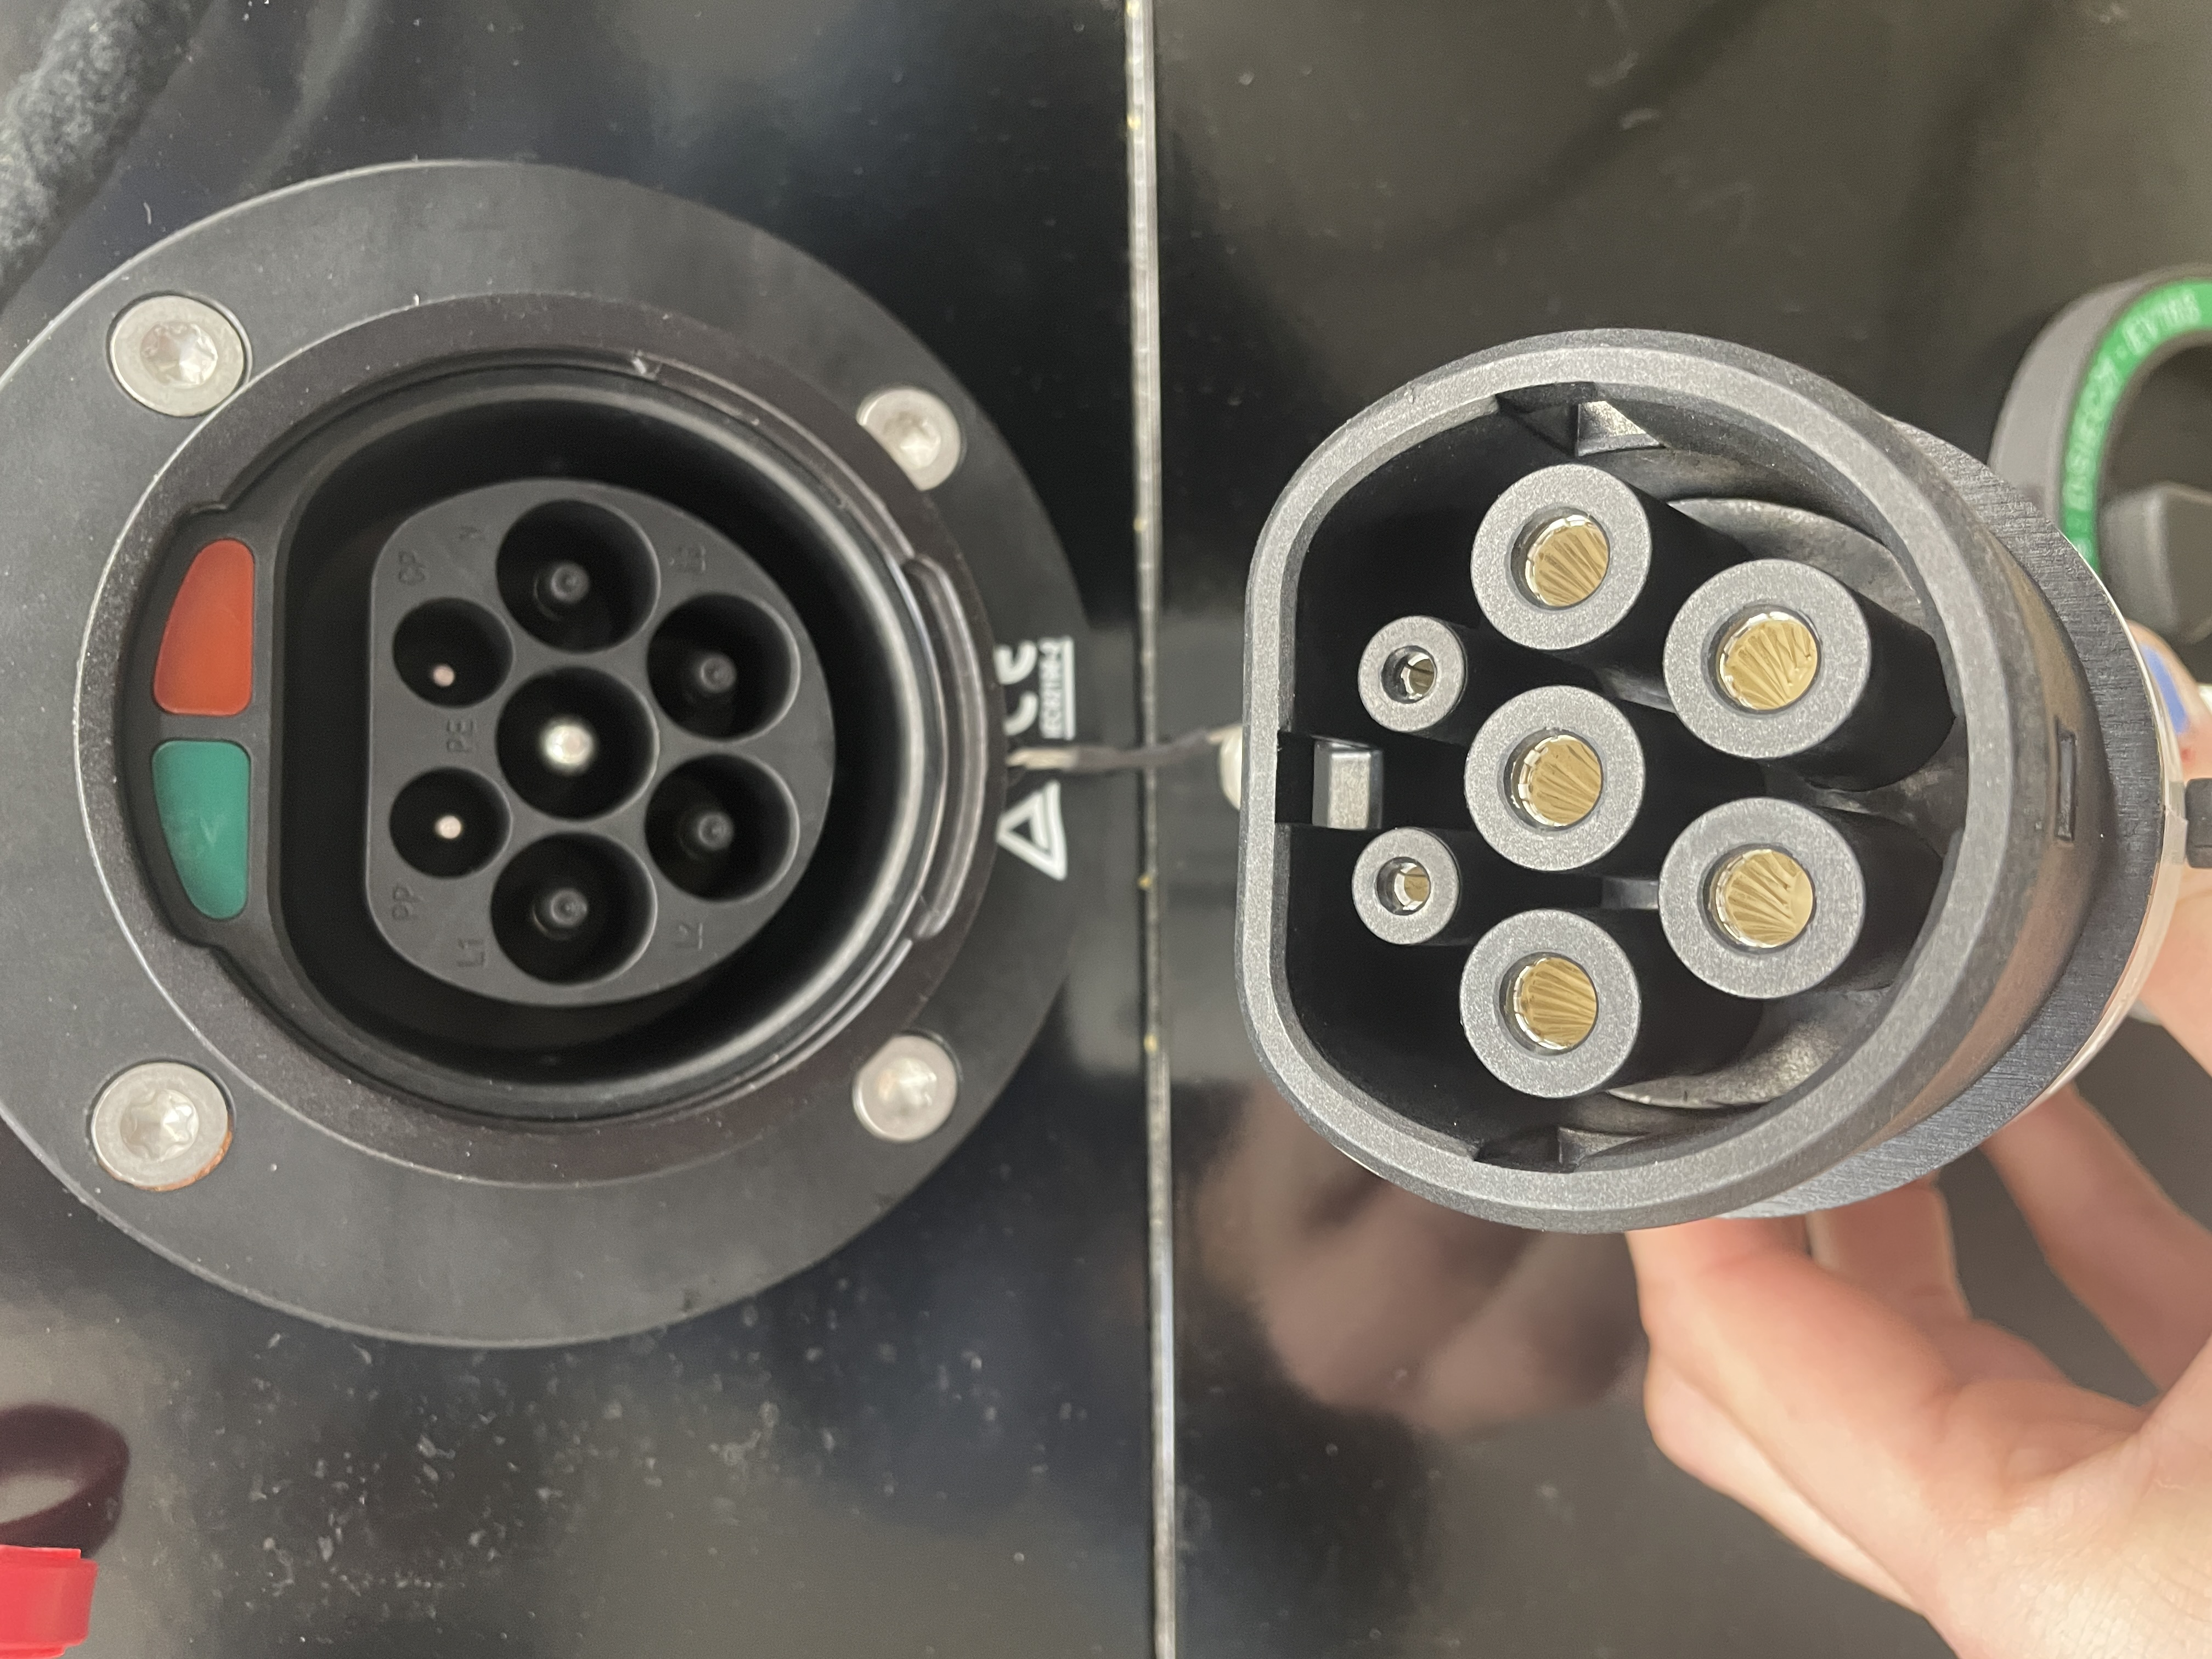
\includegraphics[width=0.9\textwidth,angle=-90]{AC_type2_inlet_outlet}}
        \caption{AC Type 2 inlet (boven) en outlet (onder)}
        \label{fig:AC_type2_inlet_outlet}
    \end{minipage}\hfill
    \begin{minipage}{0.45\textwidth}
        \centerline{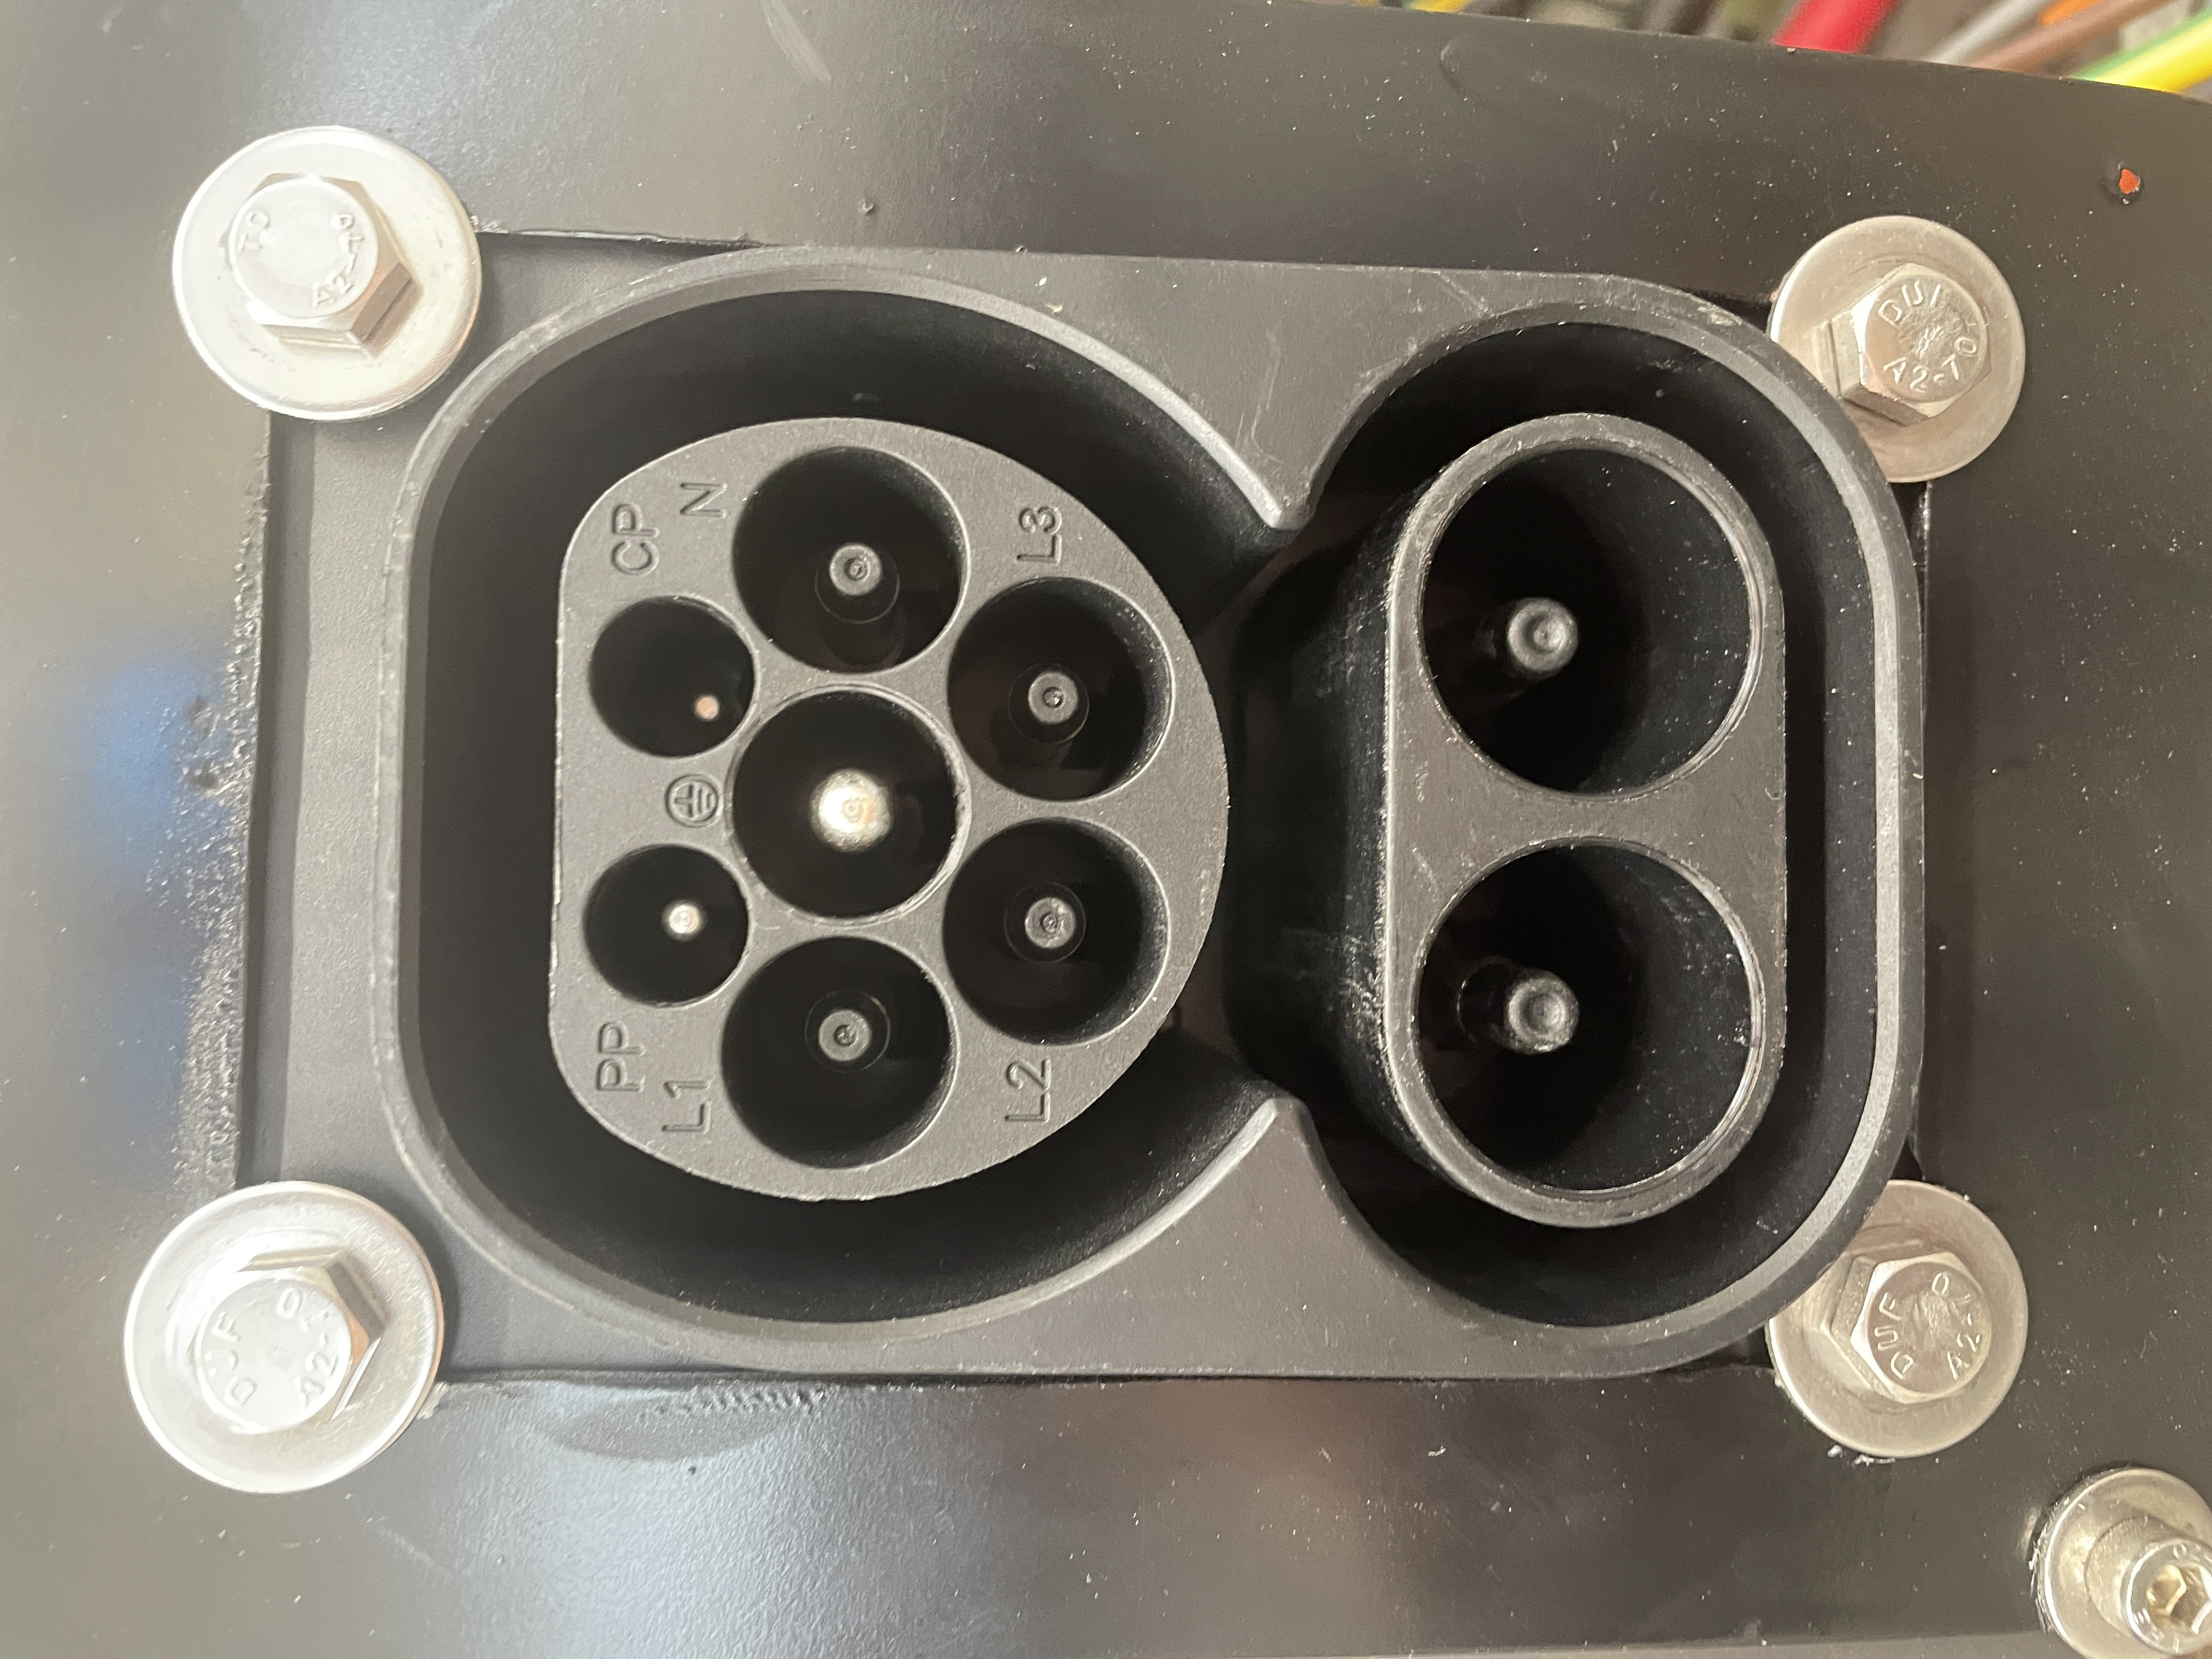
\includegraphics[width=0.9\textwidth,angle=-90]{CCS_combo2_inlet}}
        \caption{CCS Combo 2 inlet}
        \label{fig:CCS_combo2_inlet}
        \hfill
        \centerline{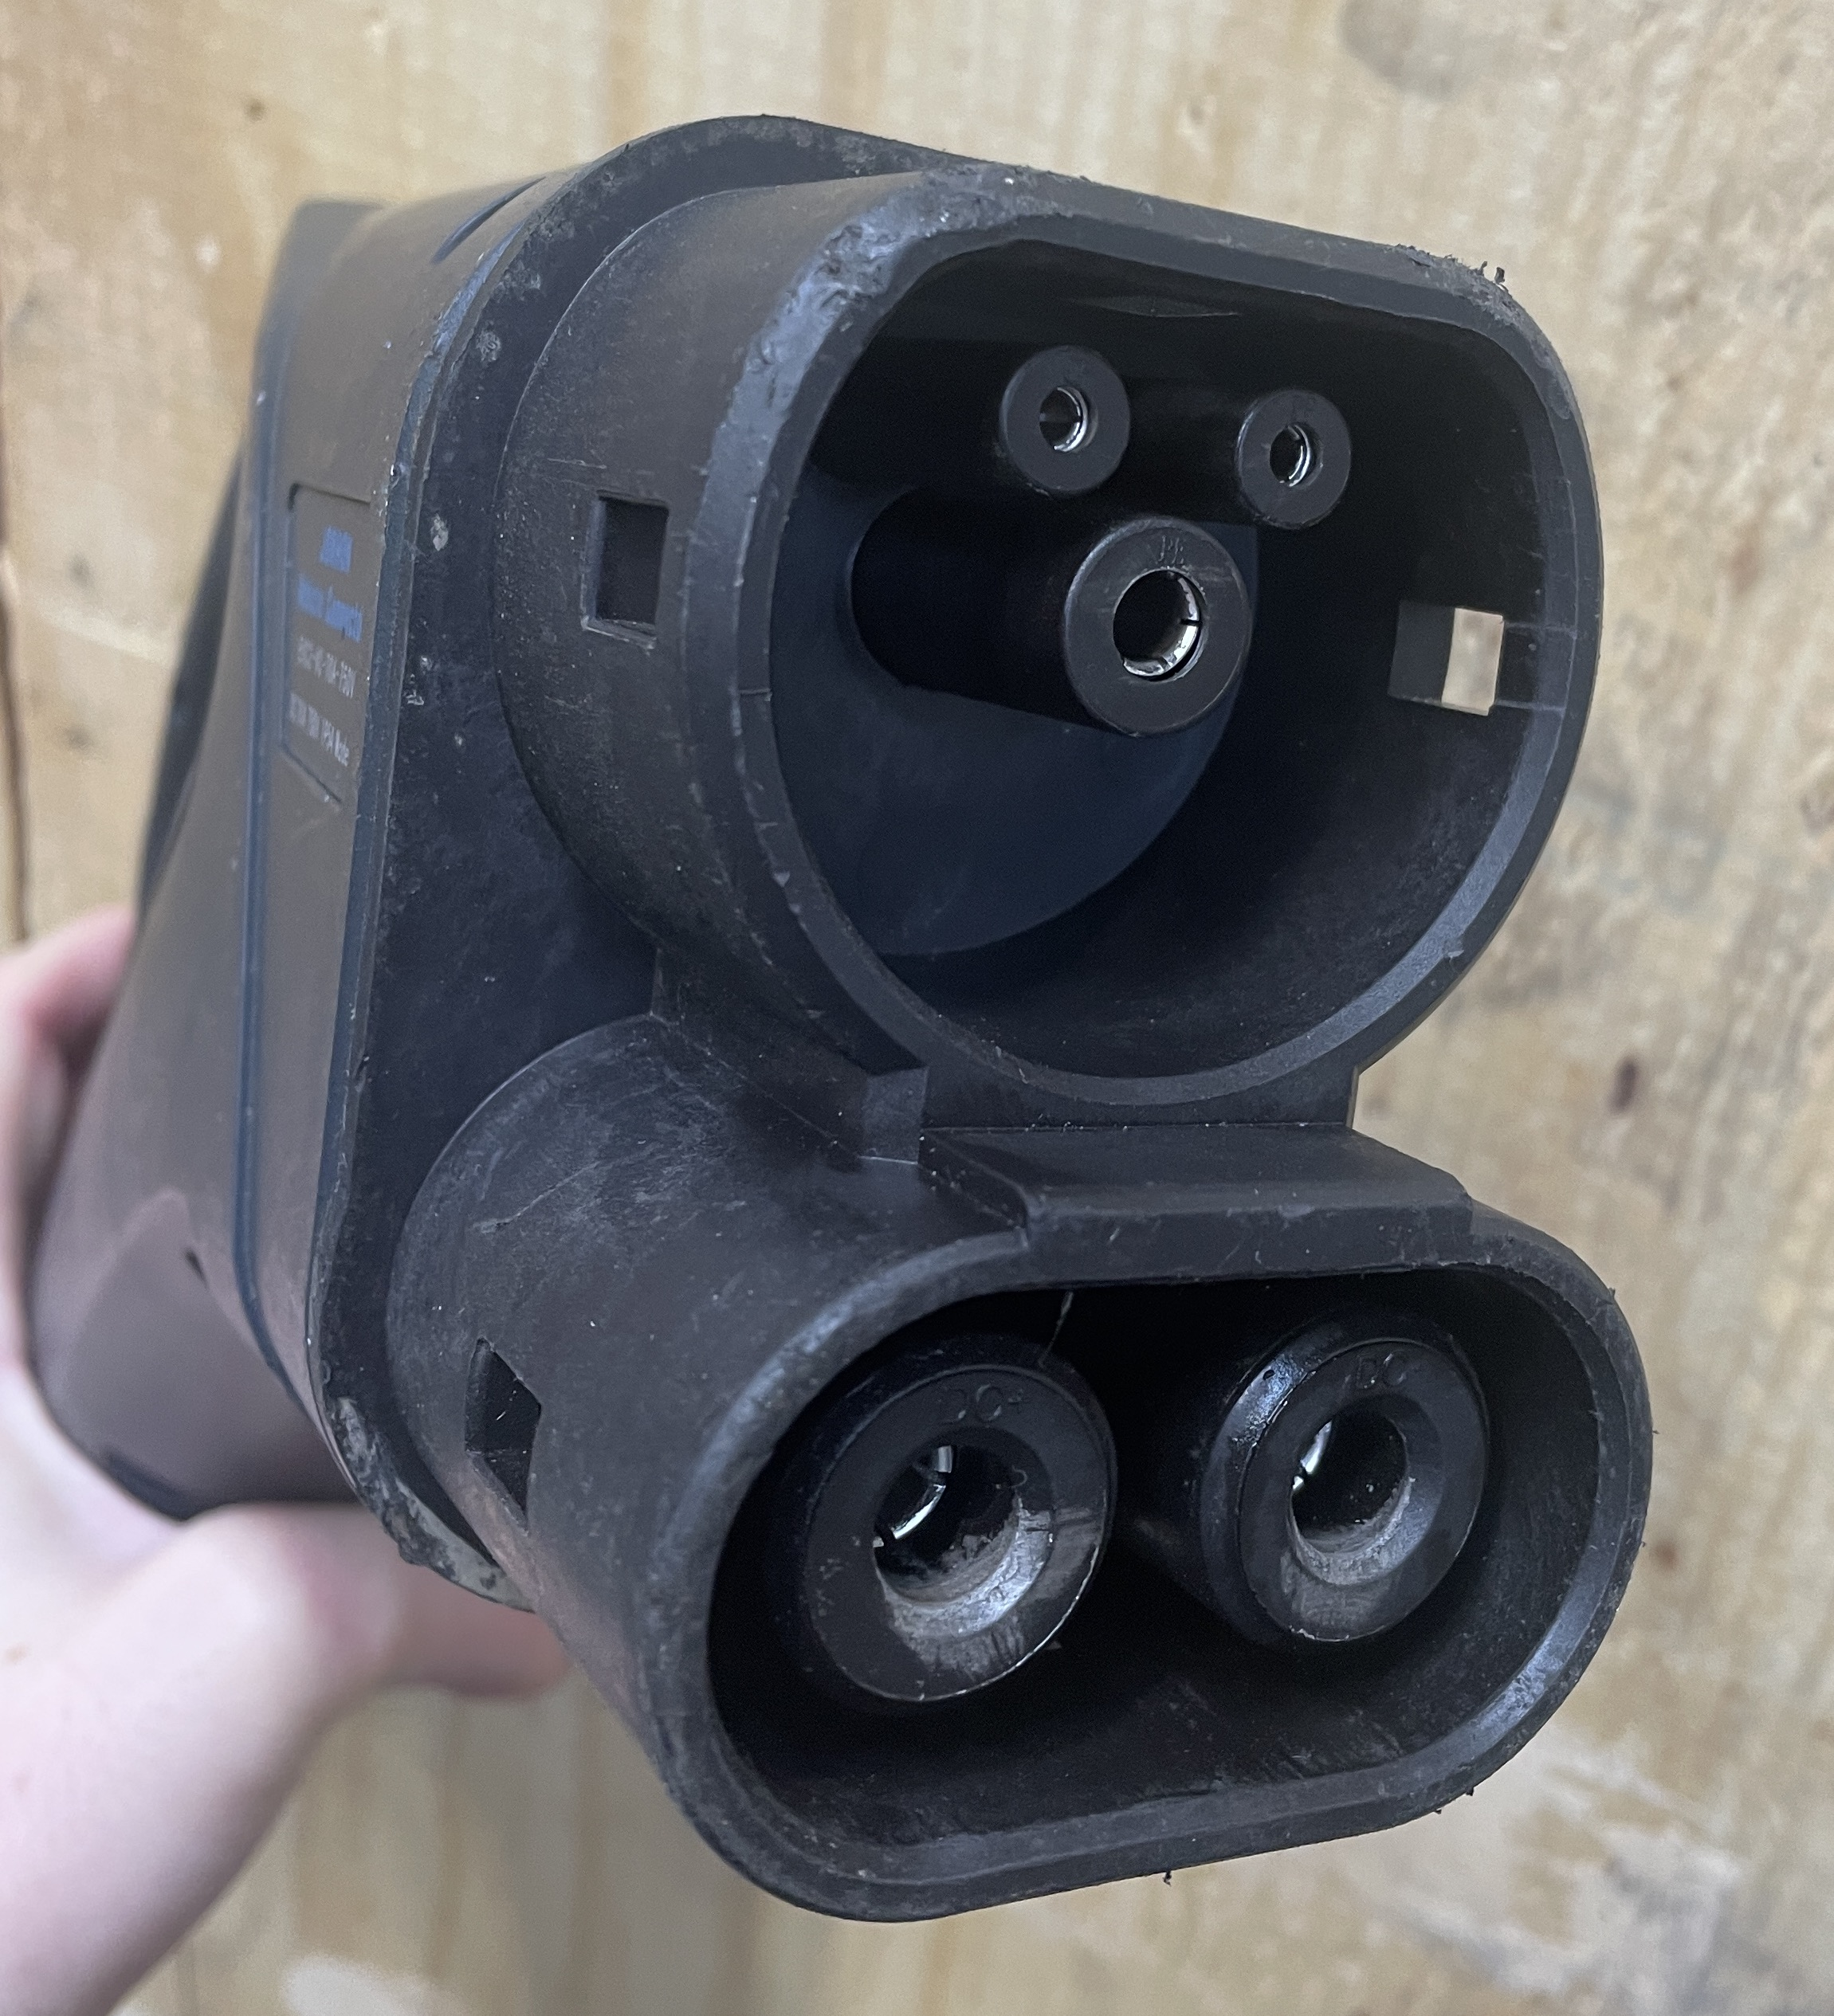
\includegraphics[width=0.9\textwidth]{CCS_combo2_outlet}}
        \caption{CCS Combo 2 outlet (stekker)}
        \label{fig:CCS_combo2_outlet}
    \end{minipage}
\end{figure}

%%%%%%%%%%%%%%%%%%%%%%%%%%%%%%%%%%%%%%%%%%%%%%%%%%%%%%%%%%%%%%%%%%%%%%%%
\subsubsection{AC laadden}
%%%%%%%%%%%%%%%%%%%%%%%%%%%%%%%%%%%%%%%%%%%%%%%%%%%%%%%%%%%%%%%%%%%%%%%%

\ac{ac} laaden kan ook nog op verschillende manieren en snelheden, het grootste
verschil is een phase en drie phase, waarbij 3 phase in princiepe drie keer
zosnel laad als een phase. Deze laadmethode gebruikt een interne laader in de
auto (\ac{ev}). En de comumicatie tussen de auto en de \ac{evse} is heel simpel
met een \ac{pwm} signal. Het \ac{pwm} signal word gebruikt om de maximale
stroom die de \ac{evse} kan leveren te comuniceren aan de \ac{ev}. De \ac{ev}
geeft dan het signal de \ac{ev} klaar is om te laaden en de \ac{evse} zet dan
netspanning op de poolen van de type 2 stekker (outlet).

%%%%%%%%%%%%%%%%%%%%%%%%%%%%%%%%%%%%%%%%%%%%%%%%%%%%%%%%%%%%%%%%%%%%%%%%
\subsubsection{DC laadden}
%%%%%%%%%%%%%%%%%%%%%%%%%%%%%%%%%%%%%%%%%%%%%%%%%%%%%%%%%%%%%%%%%%%%%%%%

\ac{dc} laaden word dus CCS laaden genoemd. De \ac{evse} gebruikt de Combo 2
outlet (stekker) en de \ac{ev} gebruikt de Combo 2 inlet (inlet). de \ac{evse}
is bij de laaden de laader, en wordt doormiddel van cantactoren in de \ac{ev}
dircet aan de accupolen aangeslooten. hiermee kan met veel hogere stroom woorde
gelaaden en daarom word \ac{dc} laaden ook wel snelladen genoemd.